
\chapter{Dinámica de redes} \label{Ch:04}

En este capítulo se comienza el estudio de las vibraciones de los átomos alrededor de sus posiciones de equilibrio y sus efectos observables. Esta llamada \textit{dinámica de redes} es necesaria para explicar propiedades como: i) la conductividad térmica de los aislantes, ii) la dependencia en $T^3$ del calor específico a baja temperatura, iii) las energías de cohesión, iv) la dilatación térmica, v) la conductividad eléctrica \textit{finita} de los metales, vi) la reflectividad de los cristales iónicos, etc.

\section{Vibraciones de los cristales con base atómica}

\subsection{La cadena lineal monoatómica}

Supongamos una cadena lineal de átomos en equilibrio. El potencial que experimenta un átomo $n$ estará modelizado de tal forma que solo depende las posiciones relativas entre este y sus átomos vecinos. En función de los vecinos que tengamos en cuenta a la hora de describir el potencial tendremos una ecuación u otra. En este caso vamos a suponer que solo tenemos en cuenta las posiciones relativas entre los \textit{primeros vecinos}. Entonces el potencial $U_n$ viene dado por

\begin{equation}
	U_n = U_n (x_n-x_{n-1},x_{n+1}-x_n)
\end{equation}
Tal y como sabemos, el punto de equilibrio de un átomo ocurre cuando el potencial está en un mínimo, denotando las posiciones de equilibrio como $x_n^0,x_{n-1}^0\ldots$ Ahora supongamos que nuestros átomos se encuentran muy cerca del equilibrio pero sin llegar a estarlo, de tal forma que:

\begin{equation}
	x_n = x_n^0 + \delta x_n
\end{equation}
de tal modo que este $\delta x_n \ll a$ siendo $a$ la distancia entre átomos en equilibrio (del orden de $\unit{\angstrom}$). A esta aproximación la llamamos \textbf{aproximación armónica}, y nos permitirá describir el potencial perturbado como un potencial armónico y por tanto describir el movimiento de los átomos/puntos de red como si fueran osciladores armónicos. En ese caso es evidente que podemos hacer una aproximación de taylor del potencial para esta posición $x_n$, de tal modo que:

\begin{equation}
	U_i (x_n)  \approx U_0 +  \parentesis{\parciales{^2U_n}{x^2}}_{x_n^0} \left\lbrace \ccorchetes{ (x_n-x_{n-1}) - (x_n^0-x_{n-1}^0) }^2 +\ccorchetes{ (x_{n+1}-x_{n}) - (x_{i+1}^0-x_{n}^0) }^2 \right\rbrace  \label{Ec:04-01-04}
\end{equation}
donde lógicamente el término de primer orden a desaparecido al encontrarse en un mínimo, El término $U_0$ es la energía en el mínimo. En este caso estamos derivando en $x$ que sería $|x_n-x_{n-1}|$ que coincide con $|x_{n+1}-x_{n}|$, ya que solo depende de la distancia relativa (que entre primeros vecinos podemos considerarla igual). Es muy importante tener claro esto, ya que de considerar más vecinos (segundos, terceros...) la derivada no será sobre la misma variable, sino que tendremos $x_1=|x_n-x_{n-1}|,x_2=|x_n-x_{n-2}|...$, generando derivadas diferentes para cada vecino considerado. Esto debe ser así ya que, como podemos ver, esta derivada segunda no es otra cosa (si lo comparamos con el potencial armónico \footnote{El potencial armónico es $U=\frac{1}{2}kx^2$ donde $x$ es el  desplazamiento relativo respecto el punto de equilibrio}) que la constante de recuperación en un muelle o lo que nosotros llamaremos \textbf{constante de fuerza}, y evidentemente la fuerza que pueda ejercer el primer vecino \textit{debe ser mayor} que la que ejerza el tercer vecino, no digamos ya el quinto. Entonces definimos la constante de fuerza $C_1$ de los primeros vecinos como:

\begin{equation}
	C_1 \equiv \parentesis{\parciales{^2U_n}{x^2}}_{x_n^0}
\end{equation}

\begin{figure}[h!] \centering
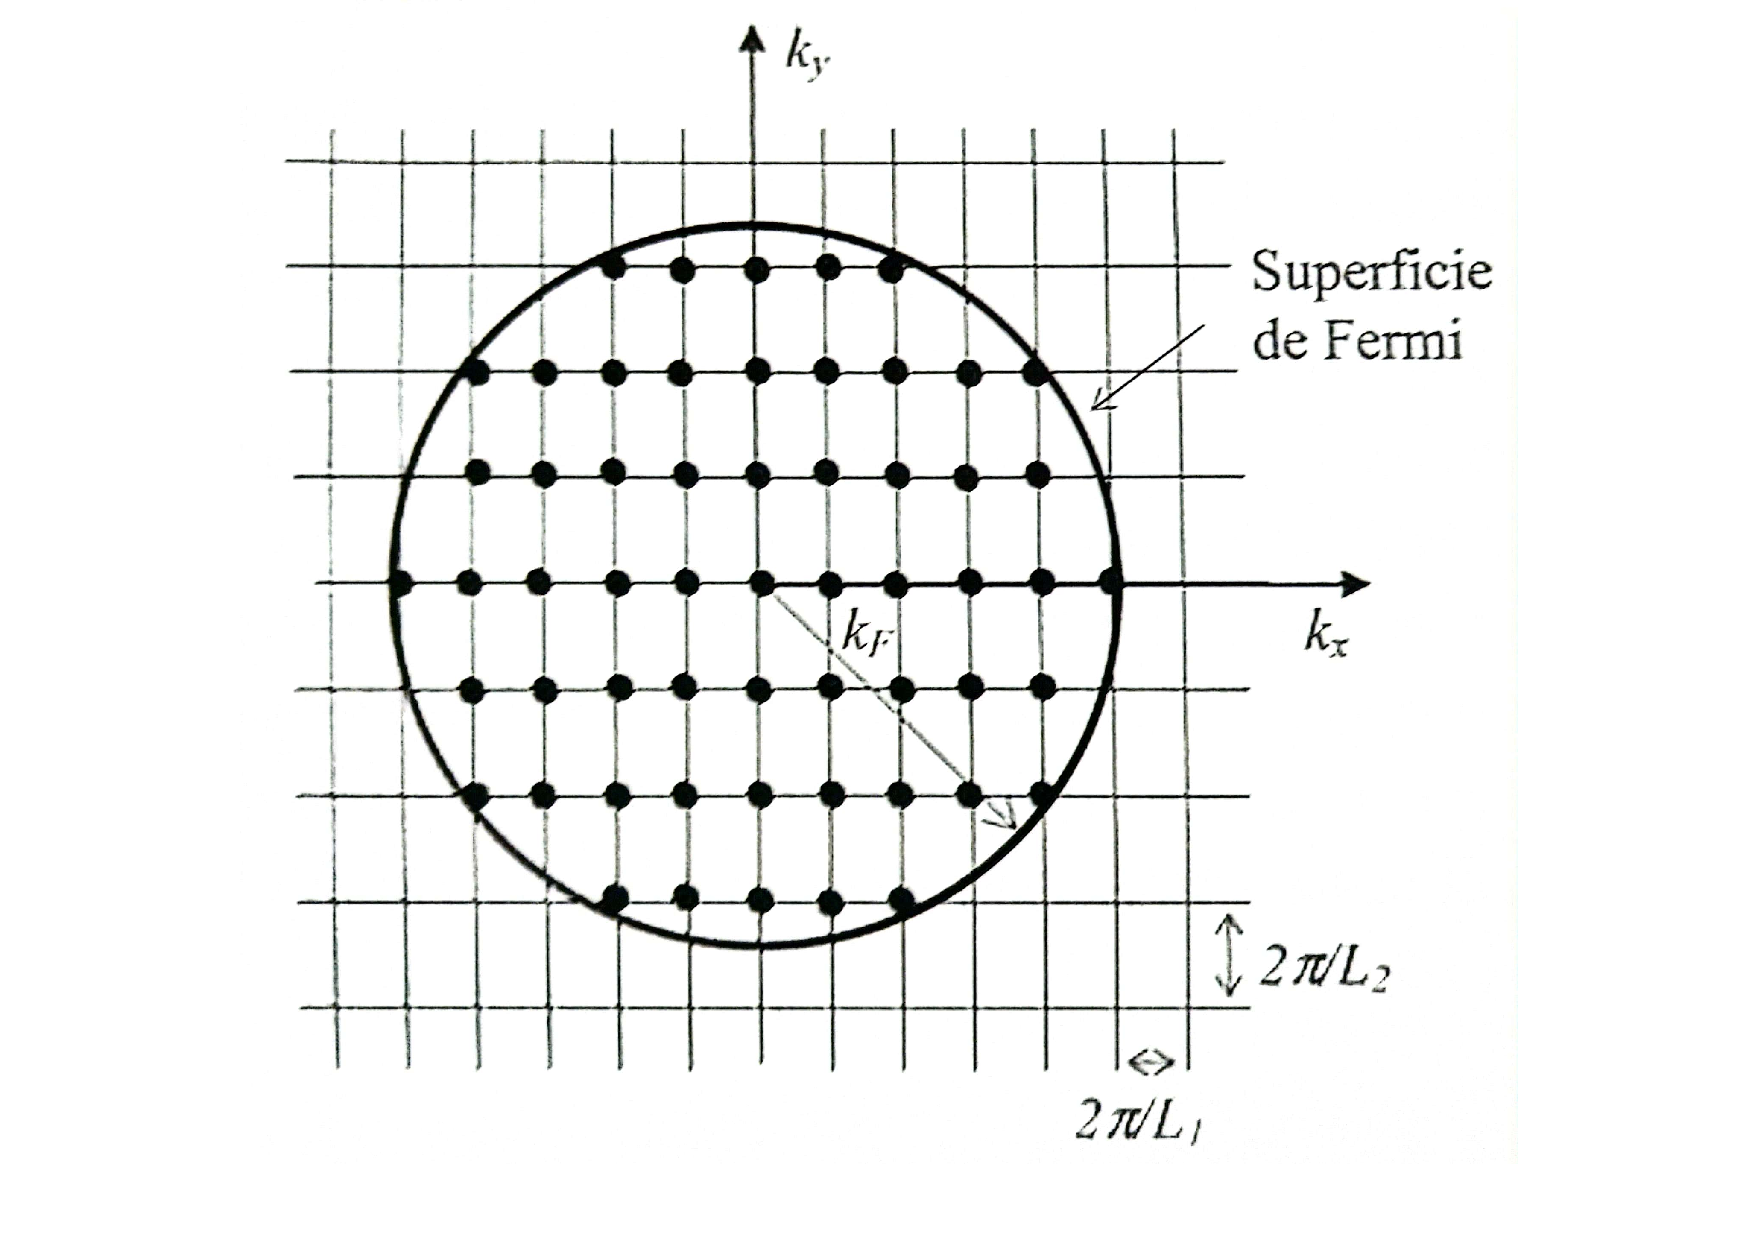
\includegraphics[scale=0.35]{Cuerpo/Ch_04/Fotos libro 1.pdf}
\caption{Parámetro de red y posiciones de átomos de masa $M$ conectados por una fuerza de constante $C$ entre planos adyacentes. Los desplazamientos de los átomos se designan por $u_{s-1},u_{s},u_{s+1}$.}
\label{Fig:04-01}
\end{figure}    

En general la ecuación anterior (\ref{Ec:04-01-04}) la podemos escribir en función de los desplazamientos infinitesimales, de tal forma que:

\begin{equation}
	U_n (x_n)  \approx U_0 +  C_1  \left\lbrace \ccorchetes{ \delta x_{n}-\delta x_{n-1}}^2 +\ccorchetes{ \delta x_{n+1}-\delta x_n}^2 \right\rbrace
\end{equation}
Una vez tenemos esto ahora solo tenemos que calcular las ecuaciones del movimiento, las cuales vendrán dadas por $m\ddot{x_n} = F_n$\footnote{Recordemos que la fuerza viene dada por el menos gradiente del potencial $\Fn=-\nabla U$}. Dado que $\ddot{x}_n=\ddot{\delta x}_n$  (la posición de equilibrio es siempre la misma), tenemos que, para cada átomo de la cadena las ecuaciones son:

\begin{equation*}
 	\vdots 
\end{equation*} 	
\begin{eqnarray}
	m\ddot{\delta x}_{n-1}  = & F_{n-1} & =  - 2C_1 \parentesis{2\delta x_{n-1}-\delta x_{n}-\delta x_{n-2}} \\
	m\ddot{\delta x}_{n}  = & F_{n}   &=  -2C_1  \parentesis{2\delta x_{n}-\delta  x_{n+1}-\delta x_{n-1}} \label{Ec:04-01-07}  \\
	m\ddot{\delta x}_{n+1}  = & F_{n+1} &=  -2C_1  \parentesis{2\delta x_{n+1}-\delta x_{n+2}-\delta x_{n}}  
\end{eqnarray}	
\begin{equation*}
	\vdots
\end{equation*}
La solución más sencilla que se nos puede ocurrir es la  \textit{solución de ondas planas} o \textit{solución armónica}:

\begin{equation}
	\delta x_n = u_k e^{i(\omega t - kx_n^0)} \label{Ec:04-01-09}
\end{equation}
donde $u_k$ no es más que la amplitud de la onda, la distancia máxima de la que se puede separar de la posición de equilibrio (recordar que $a\gg u_k$, siendo $a$ la distancia interatómica). En general la amplitud dependerá de $k$, por eso denotamos esta por $u_k$. Ahora bien, es evidente que no son válidas todas las soluciones armónicas posibles, ya que debe existir una relación entre $\omega$ y $k$. Para hallarla solo debemos sustituir (\ref{Ec:04-01-09}) en \ref{Ec:04-01-07}, y tener en cuenta que la posición de equilibrio $x_n^0 = na$:

\begin{equation*}
	m\omega^2 e^{i(\omega t -kna)} = 2C \ccorchetes{2e^{-ikna}-e^{-k(n+1)a}-e^{-k(n-1)a}} e^{i\omega t }
\end{equation*}
eliminando las exponenciales que sobran

\begin{equation*}
	m\omega^2 = 2C \ccorchetes{2-e^{ka}-e^{-ka}}   = 4C \ccorchetes{1-\cos(ka)} 
\end{equation*}
y tras una pequeña modificación, podemos llegar a que:
\begin{mybox}
\begin{equation}
	\omega = \sqrt{\frac{4C}{M}} \left| \sin \parentesis{\frac{1}{2} k a} \right| \label{Ec:04-01-10}
\end{equation}
\end{mybox}
que es llamada la \textbf{relación de dispersión} y cuya gráfica se muestra en la figura \ref{Fig:04-02}. Teniendo esto en cuenta la frecuencia máxima a la que puede vibrar la cadena es:

\begin{equation} 
	\omega_{\max} = \sqrt{\frac{4C}{m}} \label{Ec:04-01-11}
\end{equation}

La posición de la partícula $n$ viene dada por:

\begin{equation}
	x_n (t) =x_n^0 + u_k e^{-i(\omega t-k x_n^0)} =x_n^0 + u_k e^{-i(\omega t - kna)}
\end{equation}

\begin{figure}[h!] \centering
	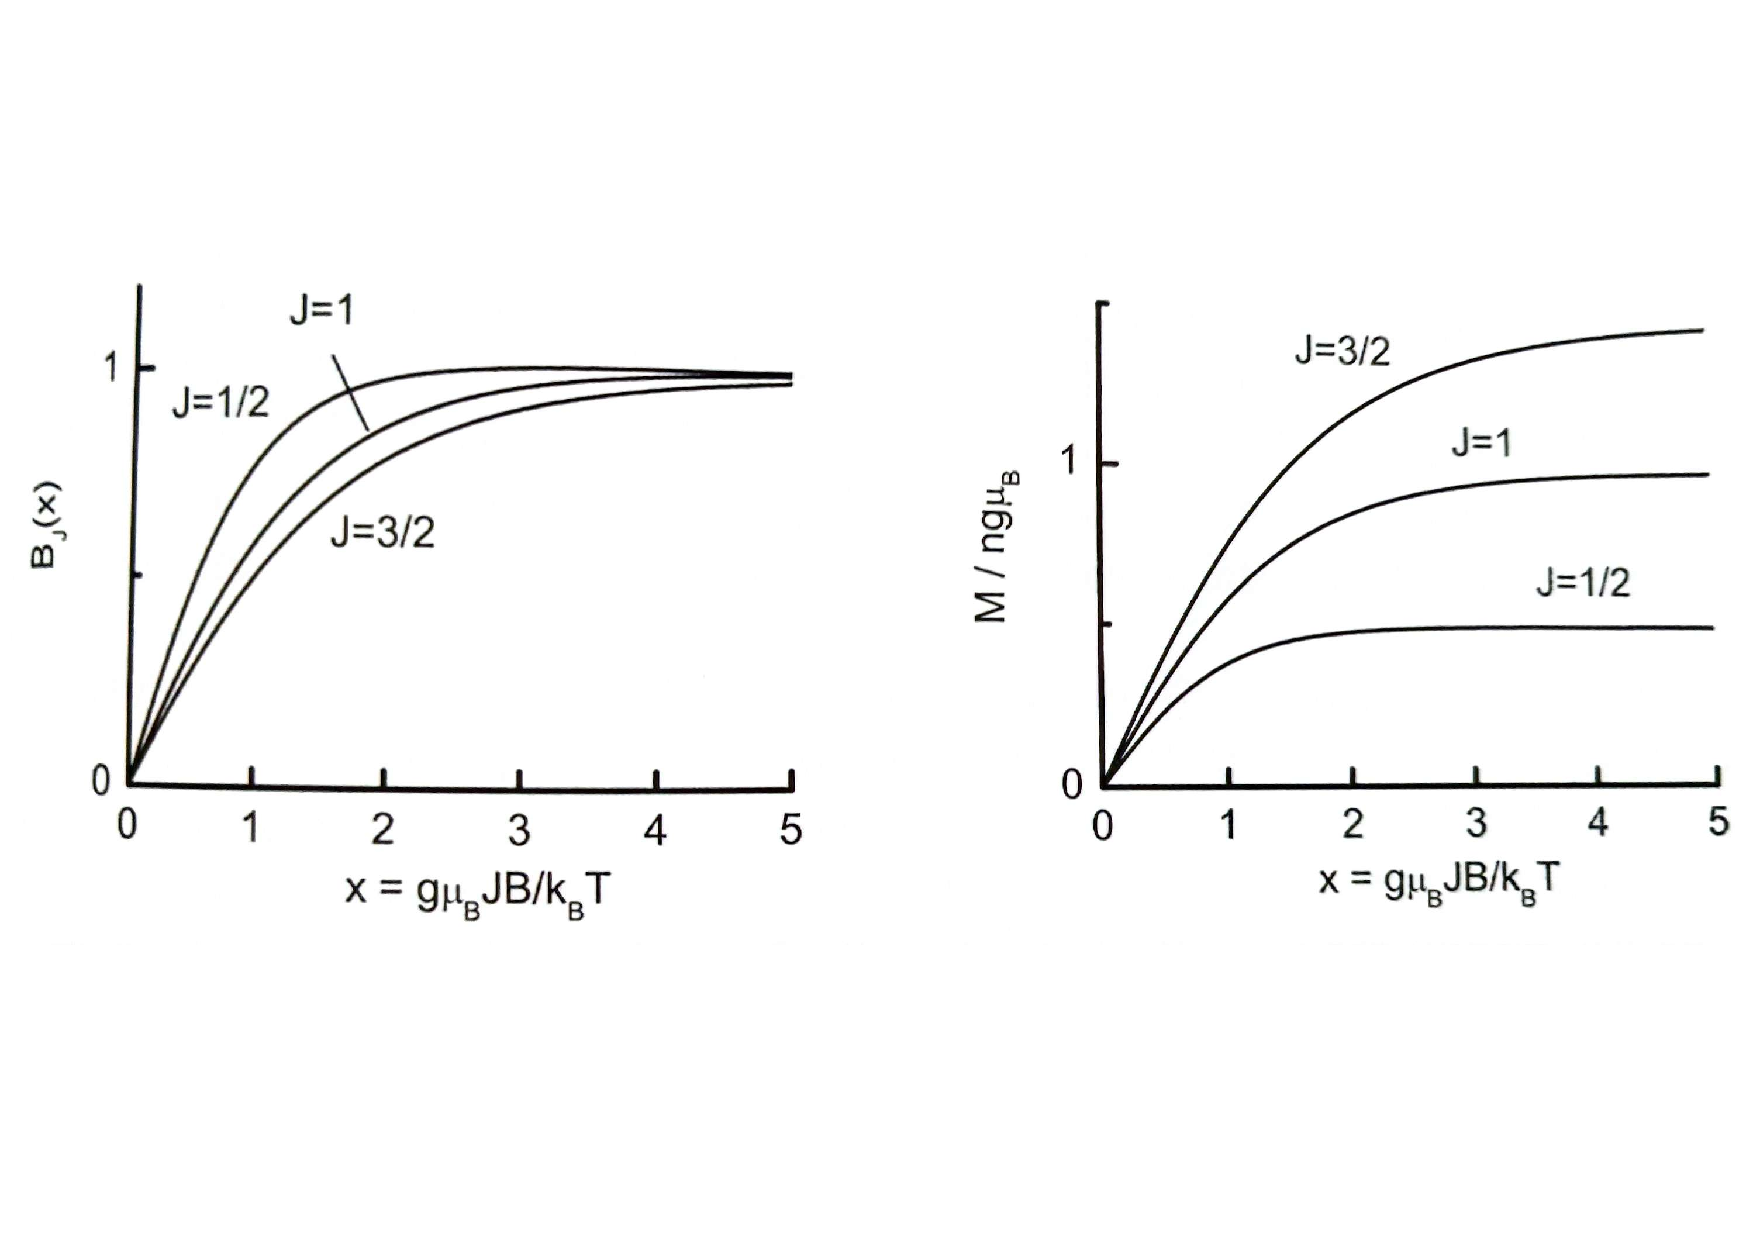
\includegraphics[scale=0.37]{Cuerpo/Ch_04/Fotos libro 2.pdf}
	\caption{Representación de la relación de dispersión de una cadena monoatómica de átomos de masa $M$ y constante de acoplamiento $C$. Observar que para $k\rightarrow 0$, $\omega \rightarrow k$}
	\label{Fig:04-02}
\end{figure}    

Una vez tenemos esto, algunos puntos importantes dentro del marco de la cadena lineal monoatómica son:

\begin{itemize}
	\item Hay simetría $k\rightarrow -k$.
	\item Hay periodicidad $k\rightarrow k+n2\pi/a=k+G$. La razón de que $k$ y $k+G$ sean equivalentes es que dan lugar a las mismas coordenadas atómicas, como se muestra con el ejemplo de la figura \ref{Fig:04-03}. Por la \textit{redundancia} existente en el espectro sólo consideramos los vectores de onda $k \in PZB$ (\textbf{primera zona de Brillouin}).
\end{itemize}

\begin{figure}[h!] \centering
    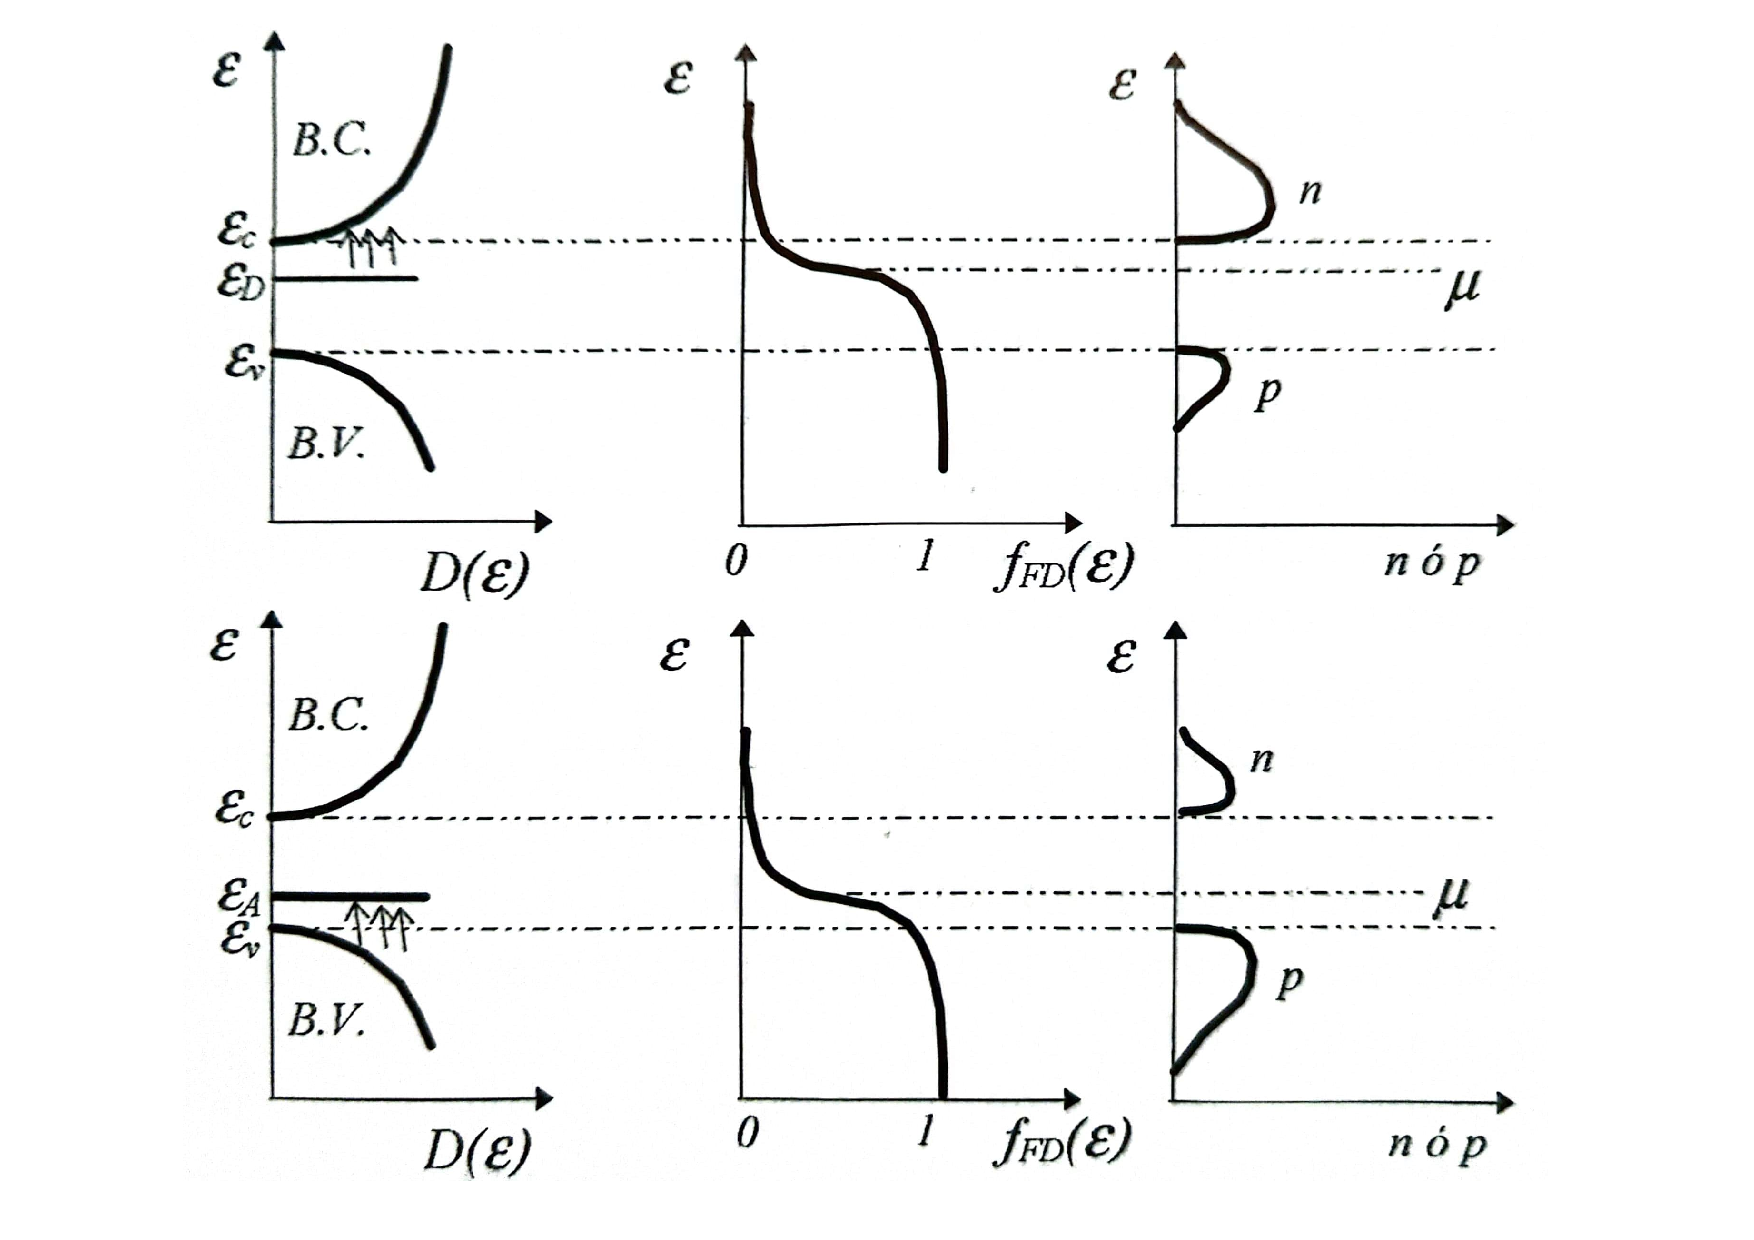
\includegraphics[scale=0.27]{Cuerpo/Ch_04/Fotos libro 3.pdf}
    \caption{Ejemplo de ondas con distinta longitud de onda que, sin embargo, representan el mismo estado de movimiento de los átomos.}
    \label{Fig:04-03}
\end{figure}    

Ahora podemos estudiar, por ejemplo, cual es la velocidad de las ondas armónicas viajando a lo largo del sólido. En general diferenciamos dos tipos de velocidades, la velocidad de fase y la velocidad de grupo \cite{Oxford_Solid_State}:

\begin{itemize}
	\item La \textbf{velociad de fase} es aquella a la que se mueve una fase concreta de la onda (esto es, a la velocidad se mueve aquella que tiene, por ejemplo, $\omega=10^{12}$ rad/s):
	
	\begin{equation}
		v_f = \frac{\omega}{k}
	\end{equation}
	\item La \textbf{velocidad de grupo} es aquella a la que se mueve el paquete de ondas, esto es, la energía. Es en general la de mayor interés, y viene dada por
	
	\begin{equation}
		v_g = \derivadas{\omega}{k}
	\end{equation}
\end{itemize}
En general la velocidad del sonido tiene una frecuencia bastante baja (y por tanto una longitud de onda muy grande). Si nos damos cuenta, para longitudes de onda grandes ($k\rightarrow 0$) la relación de dispersión (\ref{Ec:04-01-10}) es lineal (aproximación de Taylor del seno):

\begin{equation}
	\omega = \sqrt{\frac{4C}{M}} \frac{ka}{2}
\end{equation}
A toda ecuación de dispersión que verifique una relación de dispersión lineal cuando $k\rightarrow0$ la llamamos \textbf{rama acústica}. Si la dispersión es lineal la velocidad de fase y de grupo coinciden. Entonces la \textbf{velocidad del sonido} de un sólido según este modelo viene dada por:

\begin{equation}
	v_{\text{sonido}} = \sqrt{\frac{C}{M}} a
\end{equation}
sustituyendo aquí la ecuación (\ref{Ec:04-01-11}) podemos expresar la velocidad del sonido como

\begin{equation}
	v_{\text{sonido}} = \frac{ \omega_{\max} a}{2}
\end{equation}

\subsubsection{Mas allá de los primeros vecinos}

\subsubsection{Módulo de Young}

\subsubsection{Momento lineal total de la cadena}


\subsection{Cristales monoatómicos tridimensionales}

En este caso, los átomos ocupan posiciones $\rn(t) = \Rn + \un (\Rn,t)$. Si llamamos a $\phi$ al potencial de interacción entre dos átomos, la \textit{aproximación armónica} nos permite aproximar la energía total por un desarrollo en serie a segundo orden:

\begin{equation}
	U_{\text{arm}} = \frac{1}{4} \sum_{\Rn,\Rn'} \ccorchetes{\un(\Rn)-\un(\Rn')} \Phi \ccorchetes{\un(\Rn)-\un(\Rn')} \label{Ec:04-01-18}
\end{equation}
con $\Phi_{ij}=\partial^2 \phi / \partial x_i \partial x_j$, siendo $x_i(t) = R_i + u_i (\Rn,t) \ (i,j=1,2,3)$. Equivalentemente (\ref{Ec:04-01-18}) se puede escribir como:

\begin{equation}
	U_{\text{arm}} = \frac{1}{4} \sum_{\Rn,\Rn'}\un(\Rn) D(\Rn-\Rn' ) \un(\Rn') \label{Ec:04-01-13}
\end{equation}
donde 

\begin{equation}
	 D(\Rn-\Rn' ) = \delta_{\Rn \Rn'} \sum_{\Rn''} \Phi (\Rn- \Rn'') - \Phi (\Rn - \Rn')
\end{equation}
es una matriz que contiene las interacciones entre pares de átomos. La {\bf ecuación dinámica} es

\begin{equation}
 	M \derivadas{\un (\Rn)}{t^2} =  - \parciales{U_\text{arm}}{\un (\Rn)} = \sum_{\Rn'} D (\Rn-\Rn') \un (\Rn') \label{Ec:04-01-21}
\end{equation}
que admite soluciones de la forma

\begin{mybox}
\begin{equation}
	\un (\Rn,t) = \epsilonn (\Rn,t) e^{i(\kn \cdot \Rn - \omega t)}  \label{Ec:04-01-22}
\end{equation}
\end{mybox}
donde $\epsilonn(\kn)$ es el \textit{vector de polarización}. Esto no es más que la generalización de la ecuación (\ref{Ec:04-01-09}) al caso 3D. Al sustituir  (\ref{Ec:04-01-22}) en (\ref{Ec:04-01-21}) se ve que la condición de existencia de solución es 

\begin{equation}
	D(\kn) \epsilonn (\kn) = M \omega^2 (\kn) \epsilonn \kn \label{Ec:04-01-23}
\end{equation}
donde $D(\kn) = \sum_\Rn D(\Rn) e^{i \kn \cdot \Rn}$ es la llamada \textit{matriz dinámica}, que se puede ver que es real y simétrica. Esto garantiza la existencia de \textit{tres} soluciones a (\ref{Ec:04-01-23}) que verifican $\epsilonn_i (\kn) \cdot \epsilonn_j (\kn) = \delta_{ij}$, ($i,j=1,2,3$), y que se denominan \textbf{ramas acústicas} por verificarse en ellas que $\omega_i (\kn) \approx c_i (\kn)k$ para $ka\ll 1$. Dado un $\kn$, los vectores $\epsilonn$ no tienen en general que ser paralelos o perpendiculares a $\kn$. Por eso sólo se puede hablar aproximadamente de \textit{polarización longitudinal} o \textit{transversal}. A pesar de ello, los tres modos posibles para cada $\kn$ se denominan \textbf{acústica longitudinal} (LA) y \textbf{acústicos transversales} (TA). El resto de las propiedades coinciden con las del caso unidimensional.

\section{Vibraciones de cristales con base diatómica}

\subsection{La cadena lineal diatómica}

El modelo es una cadena unidimensional con base diatómica. Los átomos de la base se distinguirán por tener masa distinta (véase \ref{Fig:04-04}), aunque sería equivalente distinguirlos por sus acoplamientos. Como antes, este modelo podría representar vibraciones de cristales reales en direcciones particulares. Las ecuaciones del movimiento, admitiendo interacción sólo a vecinos más próximos y una única constante de fuerza $C$ son 

\begin{equation*}
	M_1 \derivadas{^2 u_s}{t^2} = C(v_s - u_s) + C(v_{s-1}-u_s)
\end{equation*}
\begin{equation}
	M_2 \derivadas{^2 v_s}{t^2} = C(u_{s+1} - v_s) + C(u_{s}-v_s) \label{Ec:04-02-01}
\end{equation}

\begin{figure}[h!] \centering
    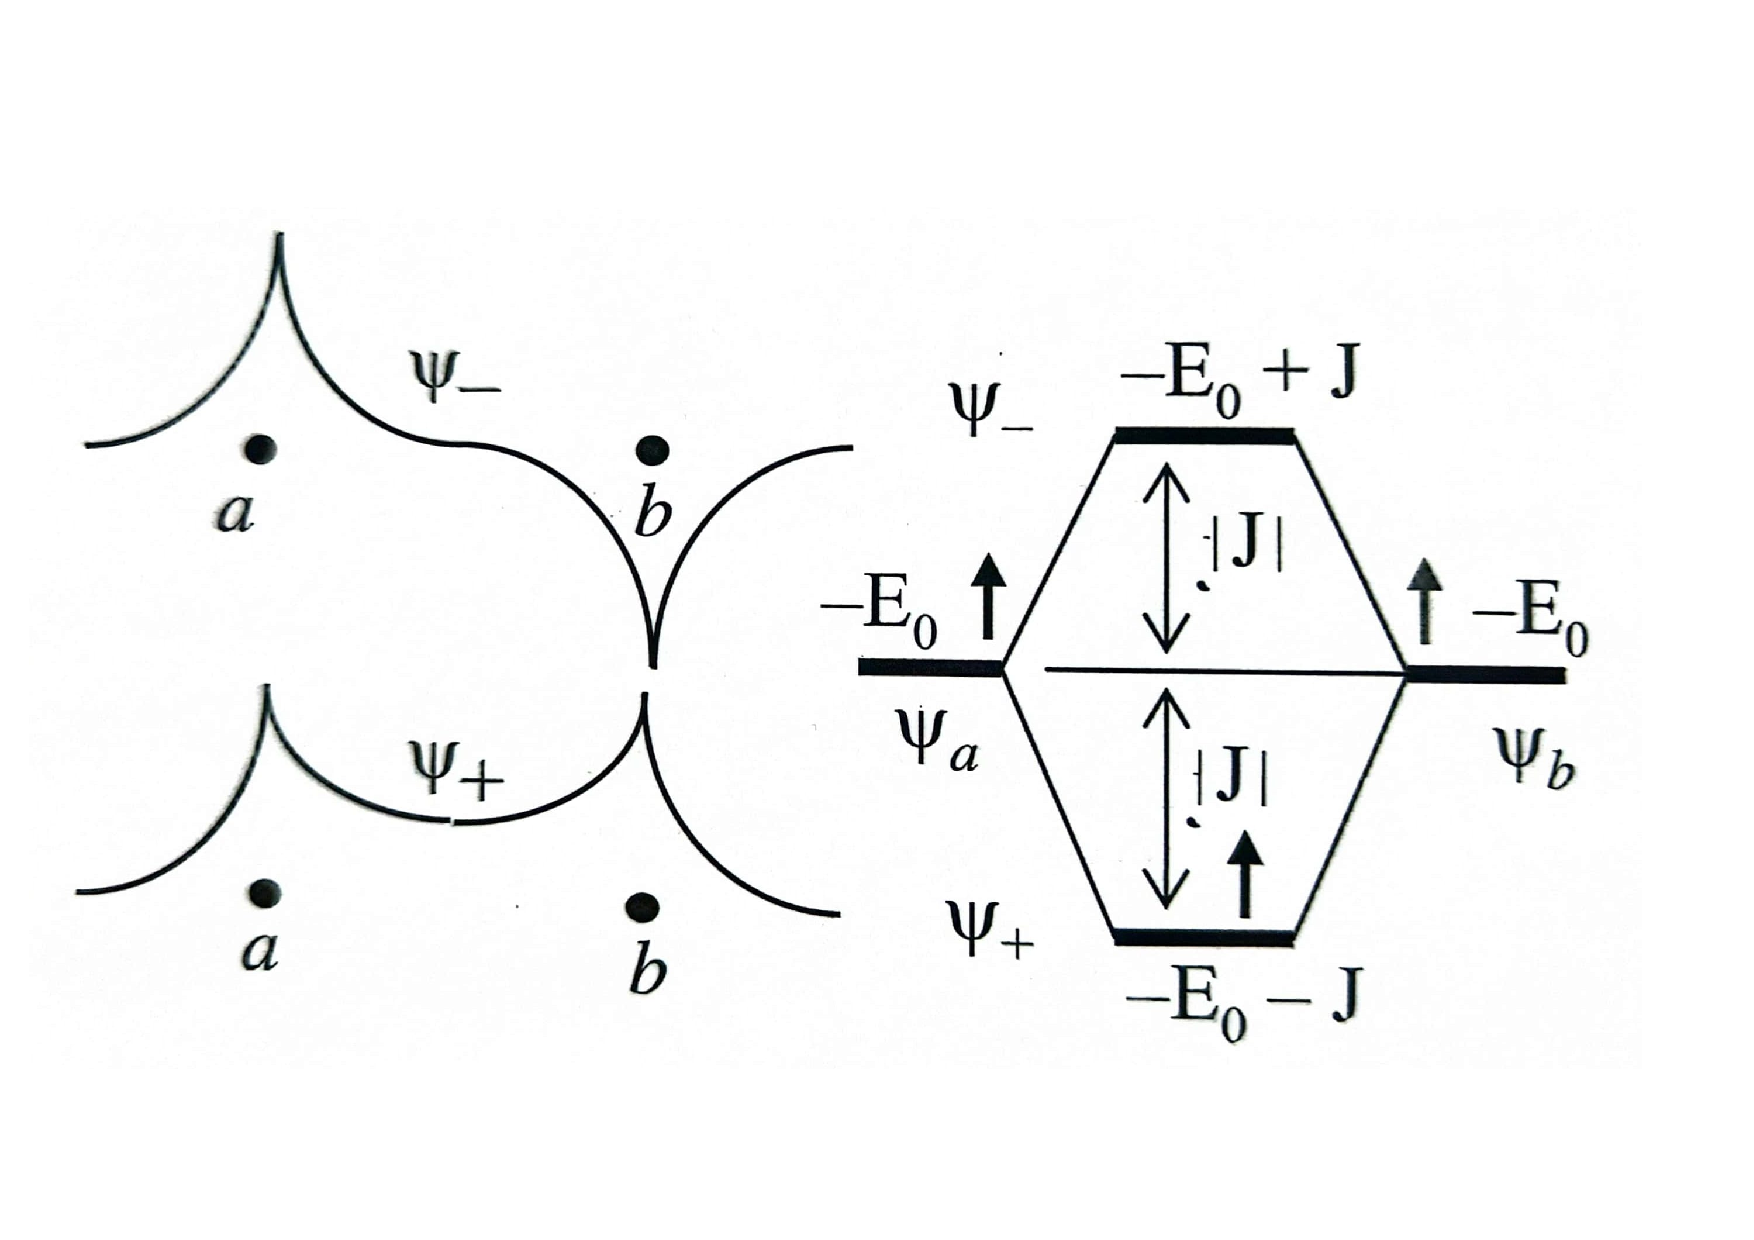
\includegraphics[scale=0.4]{Cuerpo/Ch_04/Fotos libro 4.pdf}
    \caption{Parámetro de red y posiciones de átomos 1 (masa $M_1$) y 2 (masa $M_2$) conectados por una fuerza de constante $C$ entre planos adyacentes. Los desplazamientos de los átomos 1 se designan por $u$ y los átomos 2 por $v$.}
    \label{Fig:04-04}
\end{figure}    

Una solución en modos normales, permitiendo amplitudes distintas para $M_1$ y para $M_2$ es 

\begin{equation}
	u_s = u_k e^{i(ksa-\omega  t)} \tquad v_s = v_k e^{i(ksa-\omega t)} \label{Ec:04-02-02}
\end{equation}
Al sustituir (\ref{Ec:04-02-01}) y (\ref{Ec:04-02-02}) se encuentra 

\begin{equation}
    -M_1 \omega^2 u_k = C(v_k - u_k) + C(v_k e^{-ika}-u_k)
\end{equation}
\begin{equation*}
    -M_2 \omega^2 v_k = C(u_k e^{ika} - b_k) + C(u_k - v_k)    
\end{equation*}
Para que exista una solución en $u_k,v_k$ debe verificarse que

\begin{eqnarray}
    \begin{vmatrix}
        2C - M_1\omega^2 & -C(1+e^{-ika})\\
        -C (1+e^{ika}) & 2C - M_2 \omega^2  
    \end{vmatrix}= 0 \Rightarrow \\
    \omega^2 = \frac{C(M_1+M_2)}{M_1M_2} \ccorchetes{1 \pm \sqrt{1-\frac{4M_1M_2}{(M_1+M_2)^2} \sen \parentesis{  ka/2}}}
\end{eqnarray}
El mayor cambio respecto a la cadena lineal monoatómica es que ahora existen \textit{dos modos} ($\pm$) para cada valor de $k$, como se ilustra gráficamente en la imagen \ref{Fig:04-05}. Una de las soluciones tiene las características de una \textit{rama acústica}; la otra, por corresponder, como veremos, a frecuencias próximas a las ópticas, se denomina \textit{rama óptica.}


\begin{figure}[h!] \centering
    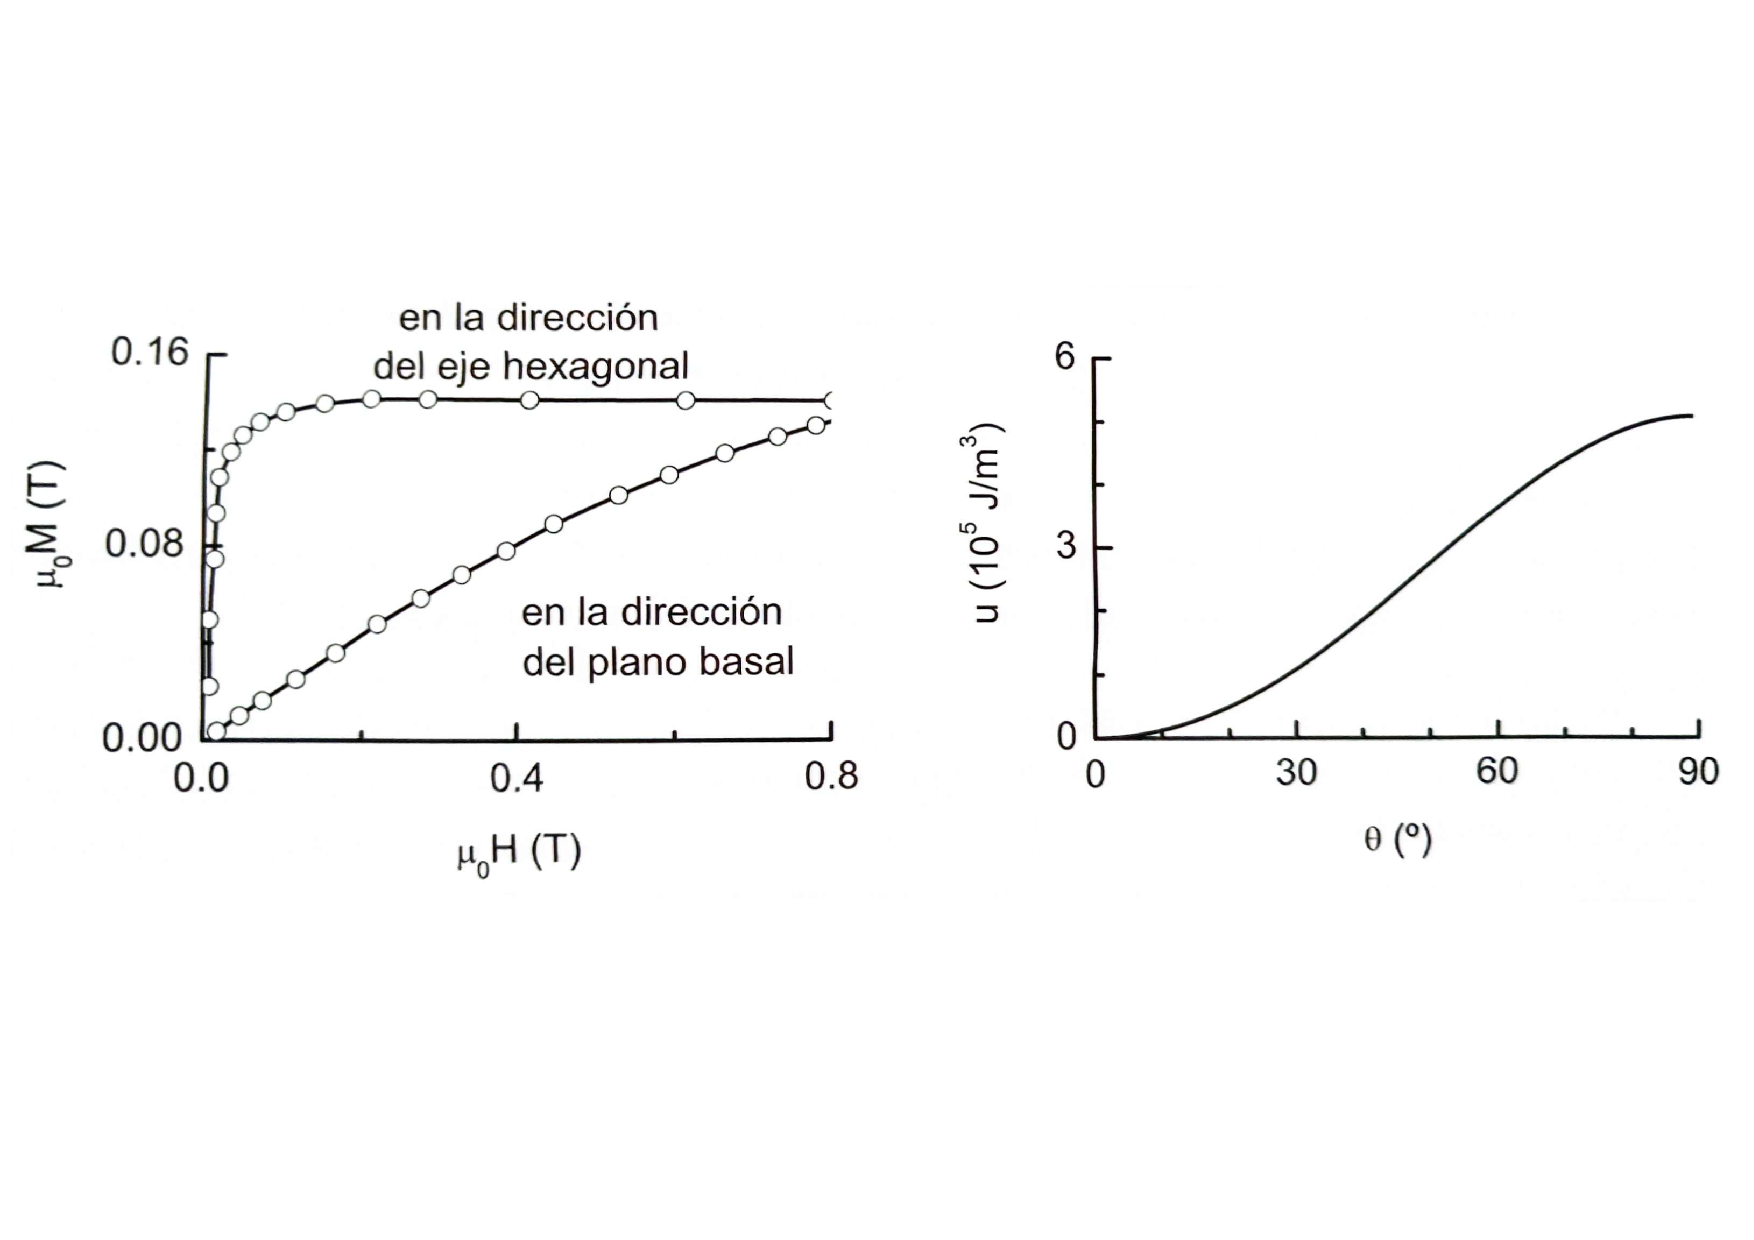
\includegraphics[scale=0.43]{Cuerpo/Ch_04/Fotos libro 5.pdf}
    \caption{Representación de la relación de dispersión de una cadena diatómica de átomos de masas $M_1$ y $M_2$ y constante de acoplamiento $C$. Observar que para la rama óptica $\omega \rightarrow \text{cte} \neq 0$ cuando $k\rightarrow 0$.}
    \label{Fig:04-05}
\end{figure}    

Es interesante excitar el tipo de movimiento atómico asociado a cada una de las ramas. Esto es especialmente sencillo si nos situamos en $ka\ll 1$, pues entonces las ecuaciones (\ref{Ec:04-02-01}) y (\ref{Ec:04-02-02}) dan $u_k/v_k=1$ para la \textit{rama acústica} y $u_k/v_k = -M_2/M_1$ para la \textit{rama óptica}. Esto quiere decir que el modo acústico los átomos de la celda se mueven en fase, es decir, la celda vibra como un todo y el movimiento es sobre todo \textit{intercelda}. En cambio, en el modo óptico los átomos se mueven en oposición de fase, de modo que el centro de masas está inmóvil y el movimiento es \textit{intracelda}. Estas características además no dependen de la aproximación $ka\ll 1$. La figura \ref{Fig:04-06} ilustra la esencia del movimiento de los modos ópticos y acústicos en el caso de un cristal diatómico. 

\begin{figure}[h!] \centering
    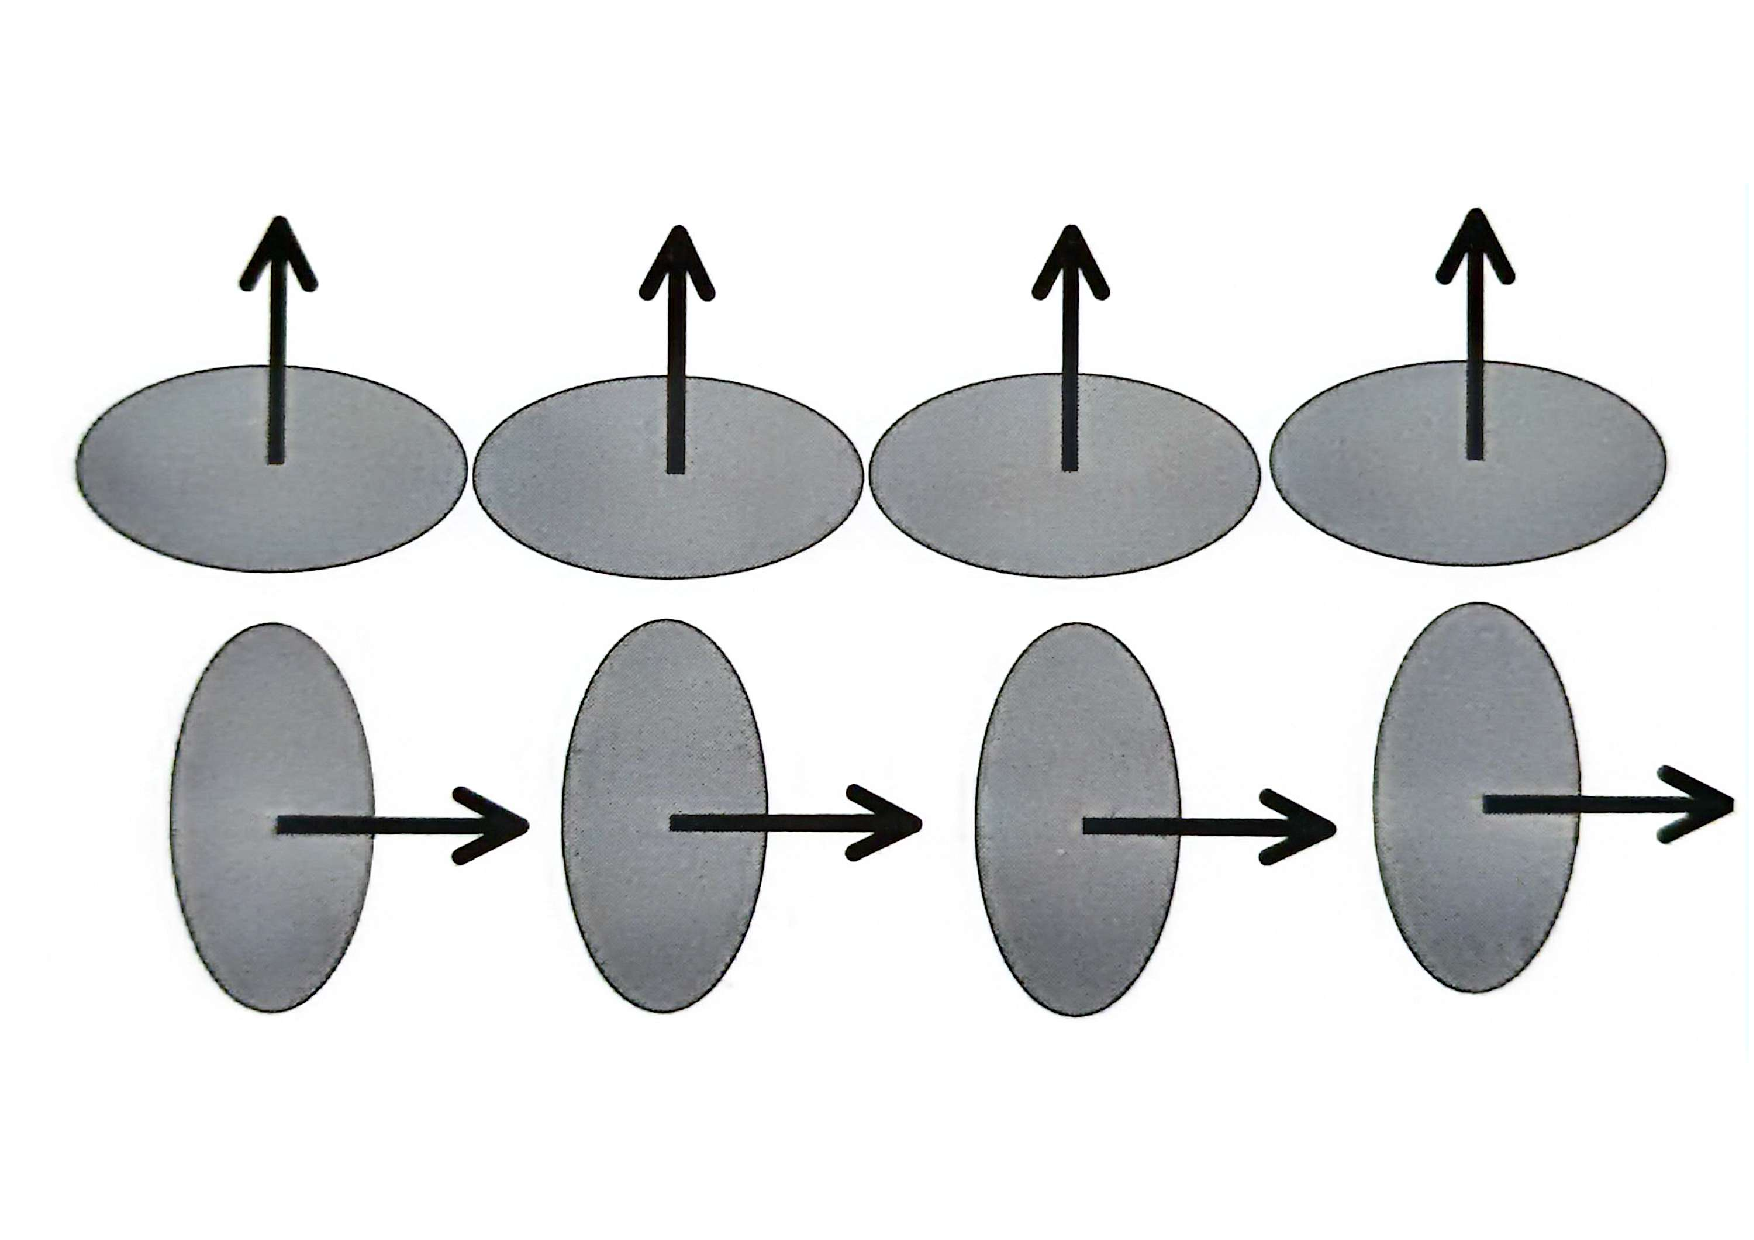
\includegraphics[scale=0.37]{Cuerpo/Ch_04/Fotos libro 6.pdf}
    \caption{Modos óptico y acústica en una cadena diatómica. El desplazamiento atómico respecto a la posición de equilibrio se representa verticalmente.}
    \label{Fig:04-06}
\end{figure}    

Obsérvense que si los dos átomos fueran iones de signo opuesto, como en un cristal iónico, cabría esperar que los modos ópticos fueran excitados por un campo eléctrico de la frecuencia adecuada. Veremos en la sección \ref{Sec:04-04} que, en efecto, existe una fuerte interacción de estos modos con las \textit{ondas e.m. infrarrojas}. Nótese finalmente, que si la cadena tuviese una base formada por $z$ átomos habría una \textbf{rama acústica} y $z-1$ \textbf{ramas ópticas}.

\begin{Anotacion}
	\textcolor{red}{Añadir imagenes de ambos movimientos pag 91-95 oxford, matrices, cadenas diatomicas con misma masa y diferente constante, explicacion zona ampliada y reducida.}
\end{Anotacion}	

\subsection{Cristales tridimensionales poliatómicos}

Como generalización (sin demostración) natural de lo que precede, se tiene que en un cristal con base de $z$ átomos existen, \textit{para cada valor de $k$, $3z$ modos normales}. Estos modos se pueden agrupar en $3z$ ramas, de las que $3$ son \textbf{acústicas} y $3z-3$ son \textbf{ópticas}. El factor 3 está asociado a las tres polarizacioens posibles y se habla de modos LA, TA, LO, TO. La figura \ref{Fig:04-07} muestra espectros de vibración de algunos sólidos simples. El punto importante es que las frecuencias características de vibración son del orden de $10^{12}$ Hz que corresponden al \textit{infrarrojo}.

\begin{figure}[h!] \centering
    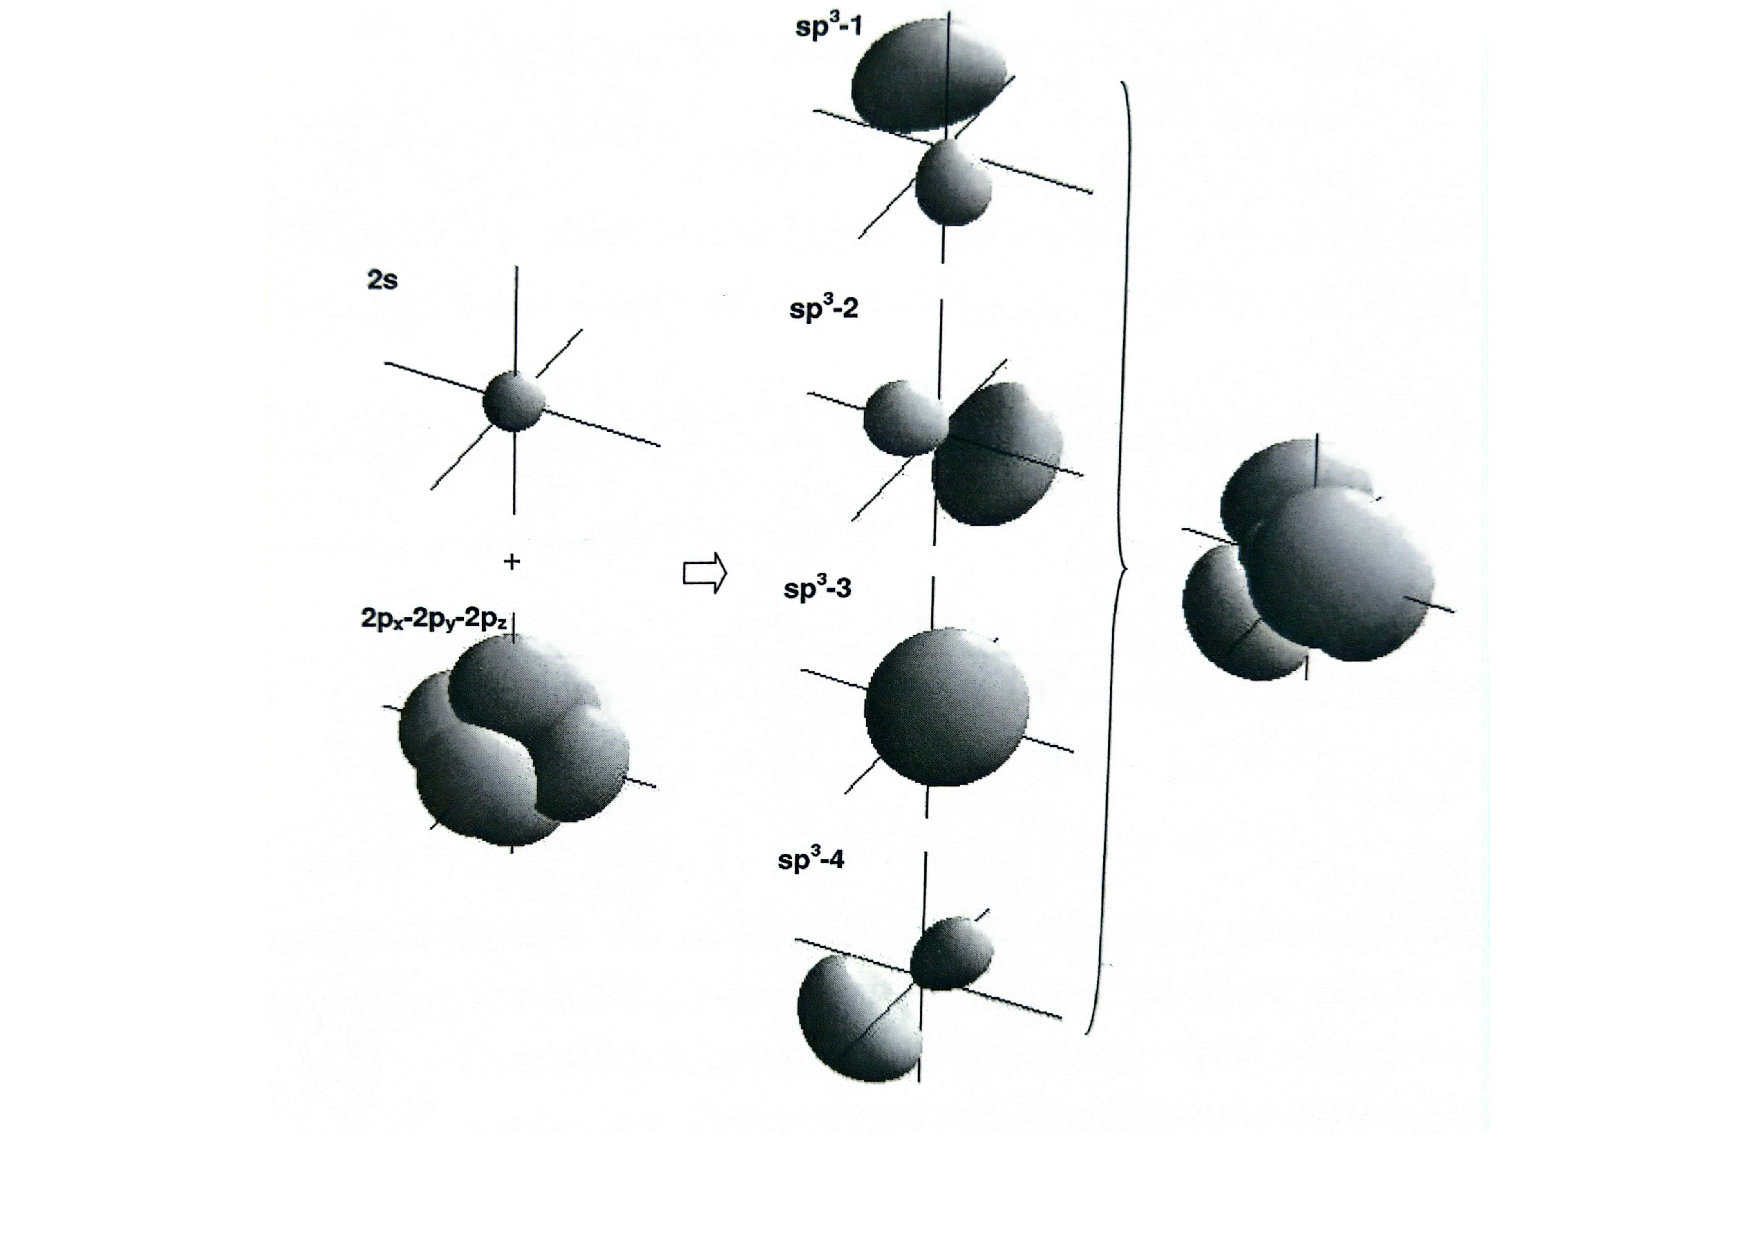
\includegraphics[scale=0.42]{Cuerpo/Ch_04/Fotos libro 7.pdf}
    \caption{Ejemplos de relación de dispersión experimental $\omega (\kn)$. En el eje horizontal se representa $\kn/\kn_{\max}$ para distintas direcciones, y en los ejes verticales la frecuencia $\omega/2\pi$ en unidades de $10^{12}$ Hz.}
    \label{Fig:04-07}
\end{figure}    

\section{Fonones}

\subsection{Cuantización de las ondas elásticas}

Para introducir el concepto de \textbf{fonón} vamos a ver una manera más formal de obtener la relación de dispersión dada por la ecuación \ref{Ec:04-01-07} haciendo uso de las \textit{variables normales}. En concreto, si se define 

\begin{eqnarray}
    \xi (k,t) & \equiv & \frac{1}{\sqrt{N}} \sum_{s=1}^N u_s (t) e^{-iksa} \\
    \Pi (k,t) & \equiv & \frac{1}{\sqrt{N}} \sum_{s=1}^N p_s (t) e^{iksa} \ \ccorchetes{\text{con} \ p_s (t) = M \parciales{u_s(t)}{t}}
\end{eqnarray}
multiplicando la ecuación del movimiento (\ref{Ec:04-01-02}) por $e^{iksa}$ y sumando a todos los valores de $s$, se encuentra que

\begin{eqnarray}
    M \parciales{}{t} \xi (k,t) & = & \Pi (k,t) \\
    \parciales{}{t} \Pi (k,t) & =  & - M \omega^2 (k) \xi (k,t)    
\end{eqnarray}c
con $\omega^2 (k) = \frac{2}{M} \sum_l C_l \sen^2 ( ka/2)$, que a primeros vecinos ($l=\pm 1$) se reduce a la ecuación \ref{Ec:04-01-07}.

Las funciones $\xi$ y $\Pi$ responden a las ecuaciones canónicas de un oscilador de masa $M$ y frecuencia $\omega$. Las soluciones ($\eta,\Pi$) se denominan \textit{modos normales} o propios del cristal. Cualquier movimiento de los átomos se pueden describir como suma de \textit{modos normales independientes} según

\begin{equation}
    u_s (t) = \frac{1}{\sqrt{N}} \sum_{k \in PZB} \xi (k,t) e^{iksa} \approx \frac{L}{2\pi \sqrt{N}} \int_{-\pi/a}^{\pi/a} \xi (k,t) e^{iksa} \D k
\end{equation}
Por tanto, un modo normal es una \textit{excitación colectiva} (involucra a todos los átomos) caracterizada por un vector de onda $\kn$ y una frecuencia $\omega$. 

La energía de cada uno de los modos posibles de vibración de un cristal está discretizada, siendo sus valores posibles los conocidos por el oscilador armónico, es decir,

\begin{equation}
    \epsilon (\kn) = \ccorchetes{n(\kn) + \frac{1}{2}} \hbar \omega (\kn)
\end{equation}
donde $n(\kn)=0,1,2,...$ es el llamado \textbf{número de ocupación}. La energía \textit{mínima} $\frac{1}{2} \hbar \omega (\kn)$ es la \textit{energía del punto cero} de cada modo. En el caso más general:
 
\begin{equation}
    \epsilon_p (\kn) = \ccorchetes{n_p(\kn) + \frac{1}{2}} \hbar \omega_p ( \kn)
\end{equation}
es decir, cada modo normal está caracterizado, además de por el vector de onda y la frecuencia, por el índice de rama, $p$. Recuérdese que para un cristal con base de $z$ átomos el número de modos por cada $\kn$ es $3z$.  

El \textit{cuanto} de energía de vibración $\hbar \omega_p (\kn)$ se denomina \textbf{fonón} y es del orden de 4 meV pues $\omega/2\pi\approx 10^{12} $ Hz. El número de ocupación es una medida de \textit{cuantos fonones} de un determinado tipo hay excitados. En la \textit{aproximación semiclásica} ($n\gg 1$) se recupera el sentido de la amplitud de oscilación $u_k$ de un modo de vector de onda $\kn$ (de la rama $p$) y entonces se verifica 

\begin{equation}
    \frac{1}{2} N M \omega_p^2 (\kn) u_p^2 (\kn) = n_p (\kn) \hbar \omega_p (\kn)
\end{equation}
Desde el punto de vista clásico, más o menos energía se traduce en mayor o menor amplitud de oscilación, mientras que el punto de vista cuántico se traduce en mayor o menor número de ocupación. 

No es difícil verificar que \textit{un modo normal no transporta impulso neto} (centro de masas del cristal inmóvil) , por lo que no cabe decir que $\hbar \kn$ es el impulso del fonón, pues entonces el impulso total del modo debería de ser $n \hbar \kn$. A pesar de esto $\hbar \kn$ del fonón verifica, en su interacción con otras partículas, \textit{leyes de conservación} similares a las del impulso habitual, como vamos a ver.


\begin{Anotacion}
	\textcolor{red}{Añadir demostración de la amplitud de onda, paginas 82-85 del Oxford, conservación del momento, numero de ocupación.}
\end{Anotacion}	

\subsection{Espectroscopía de fonones}

Supóngase un cristal monoatómico sobre el que incide una onda (neutrones, rayos x, etc.) de vector de onda $\Kn$ y de frecuencia $\Omega$. La amplitud dispersada, en la dirección $\Kn'$, por los átomos en posiciones de equilibrio $[\rn_j (t)= \Rn_j]$ es, como sabemos

\begin{equation}
    A_{\text{salida}} \propto e^{-i \Omega t } \sum_j e^{-i \Delta \Kn \cdot \rn_j} \label{Ec:04-03-09}
\end{equation}
donde $\Delta \Kn = \Kn ' - \Kn$. Supongamos ahora que existe un modo normal establecido en el cristal, de modo que las posiciones atómicas vienen dadas por $\rn_j(t) = \Rn_j + \un_j (t)$ donde $\un=\un_0  e^{\pm i \ccorchetes{\kn \Rn_j -  \omega (\kn)t}}$ . Al sustituir en (\ref{Ec:04-03-09}) se obtiene, en aproximación armónica ($u \ll R$) 

\begin{equation}
    A_{\text{salida}} \propto e^{-i\Omega t} \sum_j e^{-i\Delta \Kn \cdot \Rn_j} - i \Delta \Kn \cdot \un_0 \sum_j e^{- i (\Delta \Kn \pm \kn) \cdot \Rn_j} e^{- i \ccorchetes{\Omega \pm \omega (\kn)}t}
\end{equation}
de forma que, además de la dispersión en elástica (1\er término), tendremos \textit{dispersión inelástica} según las condiciones 

\begin{equation}
    \Omega' = \Omega \pm \omega (\kn) \tquad \Kn' = \Kn \pm \kn + \Gn
\end{equation}
Por estas relaciones de (cuasi)conservación $\hbar \kn$ recibe el nombre de \textit{cuasiimpulso}. Irradiando un cristal y examinando la radiación dispersada inelásticamente, según estas relaciones es posible conocer el espectro fonónico de un cristal $\omega (\kn)$. Entre las radiaciones más utilizadas están:

\begin{itemize}
    \item Radiación electromagnética en el rango del \textbf{\textit{infrarrojo}}: cubre $10\le k \le 10^4 \unit{cm^{-1}}$ y $10^{12} \leq \nu \leq 10^{14}$ Hz (4 meV $\leq \epsilon \leq 1$ eV). Aunque su energía es similar a la de los fonones, no lo es $\hbar \kn$ pues $k_{PZB} \approx 10^8  \unit{\cm^{-1}}$. Se utiliza por ejemplo en análisis químicos para identificar grupos funcionales dentro de las moléculas (\textit{modos ópticos}).
    \item Radiación electromagnética en el rango de la \textbf{\textit{luz visible}}: con $k\approx 10^5 \unit{\cm^{-1}}$ ($2\leq \epsilon \leq 4$ eV) se utiliza para la dispersión inelástica (\textit{espectroscopía Raman}). Aunque los cambios de energía de los fotones son muy pequeños, se pueden determinar por técnicas interferométricas. La \textit{espectroscopía Ramen} sirve para estudiar la dinámica de los electrones de conducción en metales, la naturaleza de los cristales, etc.
    \item \textbf{\textit{Neutrones}}: constituyen la sonda ideal por cuanto los \textit{neutrones térmicos} tienen tanto el vector de onda como la energía comparables a los de los fonones y de hecho la mayoría de las curvas de dispersión de fonones en sólidos se han obtenido empleando neutrones.
\end{itemize}


El espectro fonónico $\omega (\kn)$ permite obtener información muy valiosa sobre las interacciones entre átomos (alcance, intensidad, etc.) en los sólidos. Como ilustración considérese vibraciones unidimensionales incluyendo interacción de un plano con los $l$ más próximos. Como ya se ha visto la relación de dispersión es entonces
\begin{equation}
    \omega^2 (k) = \frac{4}{M} \sum_{l>0} C_l \sin^2 \parentesis{\frac{1}{2} k la}
\end{equation}
multiplicando ahora por $\cos (ksa)$ e integrando (en la $PZB$) se encuentra

\begin{equation}
    C_s = \frac{-Ma}{2\pi} \int_{-\pi/a}^{\pi/a} \omega^2 (k) \cos (ska) \D k
\end{equation}
que nos da la constante de fuerza entre cualesquiera planos atómicos a partir de $\omega (k)$.



\begin{Anotacion}
	\textcolor{red}{Añadir demostración de la ecuación de dipsersión, todo por taylor.}
\end{Anotacion}	

\section{Vibraciones de los cristales iónicos} \label{Sec:04-04}

Las oscilaciones ópticas en cristales iónicos conllevan un campo electromagnético dentro del cristal, y por tanto una interacción de largo alcance (los modos acústicos, por tratarse de movimientos de celdas neutras como un todo, no llevan asociado campo eléctrico). Por esto, \textit{el estudio de los fonones ópticos en los cristales iónicos exige estudiar simultáneamente el movimiento de iones y el campo eléctrico asociado}. Sin embargo, como las ondas electromagnéticas son transversales, el acoplamiento sólo tiene lugar para los modos ópticos transversales, que es para los que se hace este estudio. Para simplificar analizaremos sólo cristales cúbicos diatómicos (tipo CsCl, NaCL, ZnS,...) en el límite $ka\ll 1$. En estas condiciones los cristales se pueden tratar isótropicamente y macroscópicamente (medio continuo). 

Considérese una celda cualquiera con dos iones de cargas opuestas $\pm q$. Representemos por $u_+$ $u_-$ los desplazamientos locales de sendos iones, y por $M_+$ y $M_-$ sus masas. En el límite $ka\ll 1$ todos los iones del mismo signo en la vecindad de la celda considerada se moverán al unísono de modo que las ecuaciones del movimiento son:

\begin{eqnarray}
	M_+ \parciales{^2 \un_+}{t^2} & = & 2C(\un_- - \un_+) + q \En \label{Ec:04-04-01}\\
	M_- \parciales{^2 \un_-}{t^2} & = & 2C(\un_+ - \un_-) - q \En \label{Ec:04-04-02}
\end{eqnarray}
donde se ha incluido la \textit{interacción de largo alcance} a través del campo eléctrico. 

Introduciendo la coordenada relativa $\wn = \un_+ - \un_-$ en las ecuaciones (\ref{Ec:04-04-01}) y (\ref{Ec:04-04-02}) dan

\begin{equation}
	M^* \parciales{^2 \wn}{t^2} = - M^*  \omega_0^2 \wn + q \En \label{Ec:04-04-03}
\end{equation}
con $M^*=M_+M_-/(M_++M_-)$ y $\omega_0=(2C/M^*)^{1/2}$, que sería la frecuencia de los modos ópticos, tanto longitudinales como transversales, para $ka\ll 1$, suponiendo fuerzas de corto alcance. 

Una solución ondulatoria a (\ref{Ec:04-04-03}) , es decir, con $\wn\propto e^{-i\omega t}$, permite, al sustituir, despejar

\begin{equation}
	\wn = \frac{q\En}{M^* (\omega_0^2 - \omega2)}\label{Ec:04-04-04}
\end{equation}
Por (\ref{Ec:04-04-04}) es obvio que $\wn$ es función del campo eléctrico, pero a su vez el campo eléctrico $\En$ tiene su origen en $\wn$. Esto se puede ver recordando que la \textit{polarización} $\Pn$, está ligada al campo eléctrico a través de la permitividad $\epsilon (\omega)$ según 

\begin{figure}[h!] \centering
	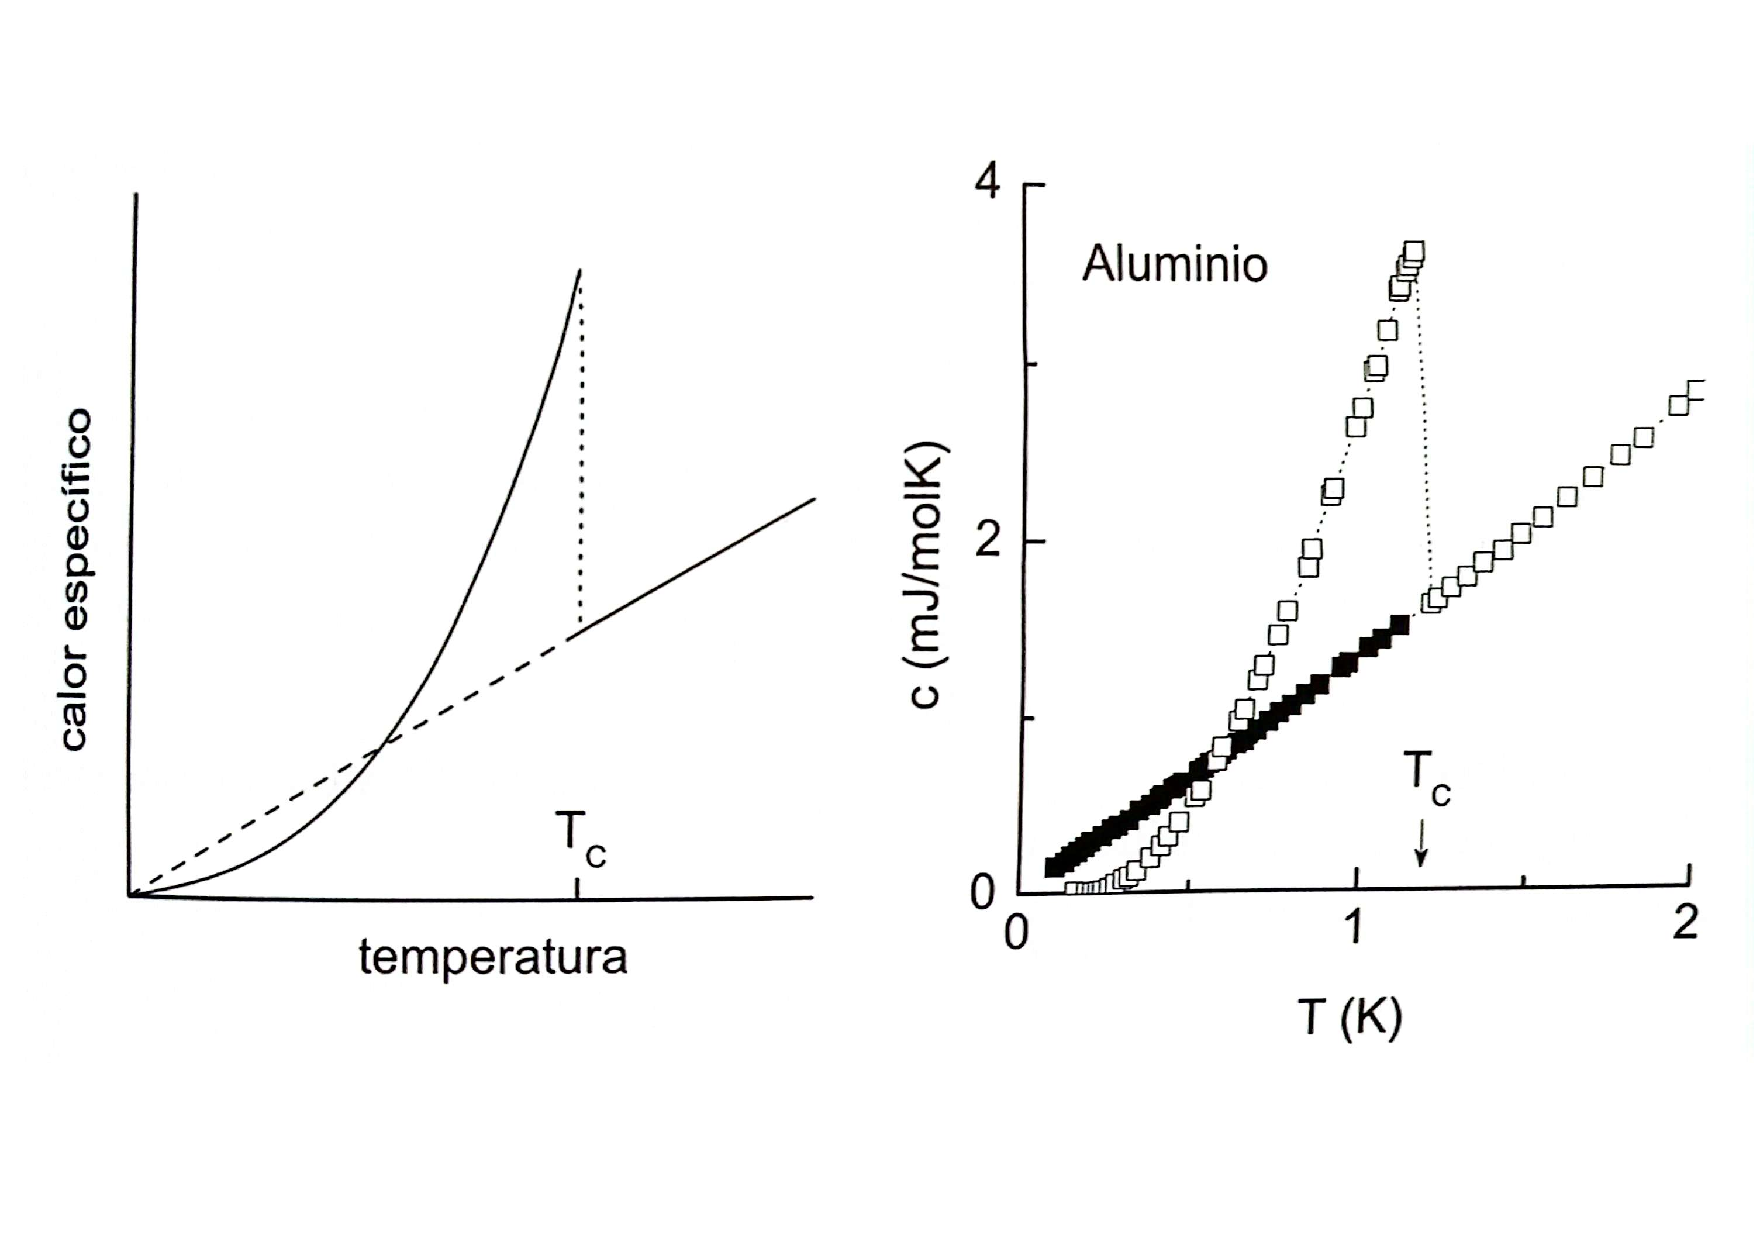
\includegraphics[scale=0.4]{Cuerpo/Ch_04/Fotos libro 8.pdf}
	\caption{(a) Dependencia con la frecuencia de la permitividad eléctrica relativa en cristales iónicos. (b) reflectividad de algunos cristales iónicos para longitudes de odna en el rango infrarrojo.}
	\label{Fig:04-08}
\end{figure}    


\begin{equation}
	\Pn = \ccorchetes{\epsilon (\omega) -1 } \epsilon_0  \En
\end{equation}
y observando por otro lado que, la definición de \textit{polarización} como una \textit{densidad de momento dipolar}, se tiene  

\begin{eqnarray}
	\Pn = n q (\un_+ - \un_-) + \Pn_\infty
\end{eqnarray}
Aquí $n$ denota el número de celdas por unidad de volumen y 

\begin{equation}
	\Pn_\infty = \ccorchetes{\epsilon (\infty) -1 } \epsilon_0 \En\label{Ec:04-04-07}
\end{equation}
es la contribución a $\Pn$ de las nubes electrónicas [la notación $\epsilon (\infty)$ indica que esta contribución se refiere a $\epsilon (\omega)$ a frecuencias electrónicas muy grandes (comparadas con las de la vibración reticular)]. Combinando (\ref{Ec:04-04-04}) y (\ref{Ec:04-04-07}) se obtiene que

\begin{equation}
	\epsilon(0) = \epsilon(\infty)  + \frac{nq^2}{\epsilon(0) M^*\omega_0^2}
\end{equation}
resulta 

\begin{equation}
	\epsilon (\omega) = \epsilon(\infty) + \ccorchetes{\epsilon(0)-\epsilon(\infty)} \frac{\omega_0^2}{\omega_0^2 - \omega^2} \En\label{Ec:04-04-09}
\end{equation}
cuya gráfica se muestra en la figura \ref{Fig:04-08} (a). En ella $\omega_L$ es la frecuencia para la que $\omega(\omega_L)=0$, que por  (\ref{Ec:04-04-09}) verifica $\omega_L = (\epsilon(0)/\epsilon(\infty))^{1/2} \omega_0 >\omega_0$.


Los rasgos esenciales del comportamiento de la luz frente a los cristales iónicos se puede deducir de comparar la relación de dispersión (\ref{Ec:04-04-09}) con la general para ondas electromagnéticas trasversales, esto es,

\begin{equation}
	\omega = k \frac{c}{\sqrt{\epsilon(\omega)}} \tquad (c = \text{velocidad de la luz})	\label{Ec:04-04-10}
\end{equation}
Para $\omega_0 < \omega < \omega_L$, $\epsilon <0$ y por (\ref{Ec:04-04-10}) $k$ es complejo puro: $k \propto i \alpha$, con lo que la onda con la parte espacial $E \propto e^{ika} = \epsilon{\alpha x}$ se amortigua exponencialmente, es decir, hay una fuerte \textit{atenuación}. También $\epsilon (\omega \rightarrow \omega_0) \rightarrow \infty$ lo que conlleva una reflectividad $r= (\sqrt{\epsilon(\omega)}-1)^2 / (\sqrt{\epsilon(\omega)}-1)^2$ que se acerca a la unidad, de acuerdo con lo que ses observara experimentalmente, como se ilustra en la imagen \ref{Fig:04-08} (b). Como $\omega_0\approx 2 \pi \times 10^{12} \unit{rad \ s^{-1}}$, la alta reflectividad tiene lugar en el \textit{infrarrojo}, lo cual se utiliza tanto para determinar experimentalmente $\omega_0$ como para producir radiación muy monocromática en el infrarrojo mediante sucesivas en cristales iónicos.

\begin{Anotacion}
	\textcolor{red}{Añadir ejercicios (ej 10)}
\end{Anotacion}
